%3.2.tex

LLVMには自動ベクトル化機能が備わっている.
自動ベクトル化とは配列の演算処理などのループによる繰り返し処理をベクトル命令の形式に置き換える機能である.LLVMによる自動ベクトル化機能はソースコードにおけるループをベクトル化されたLLVM IRへと変換が行われる.
LLVMによる自動ベクトル化の例を図\ref{fig:LLVM_auto_vec}に示す.
LLVM IRにおいてベクトル命令はベクトル型を用いて表現される.図\ref{fig:LLVM_auto_vec}にて$<$128 x i32$>$となっている箇所がベクトル型の指定を行っており,これは128個の32ビット整数の演算を行うベクトル型の命令となっている.

\begin{figure}[b]
    \centering
    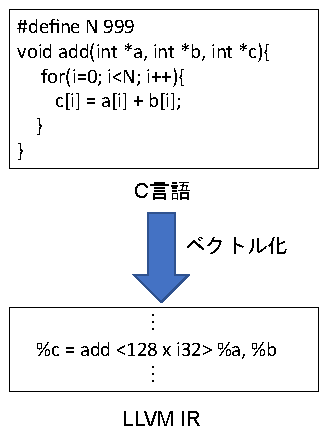
\includegraphics[scale=0.7]{image/Auto_vectorize.pdf}
    \caption{LLVMによる自動ベクトル化例}
    \label{fig:LLVM_auto_vec}
\end{figure}

%また,LLVM IRにおけるベクトル処理の流れを図%フローチャートを作って載せる
%に示す.
また,LLVM IRでは対象の全データに演算を行うための制御を行っている.例えば対象データ要素数が400とし,一度にベクトル演算を行う個数を128とする.この場合,128個を対象としたベクトル演算を3回行う.するとベクトル演算では384個の要素を演算することができるが,16個の要素が余っている.このあまりに関しては逐次処理によってスカラ演算を16回繰り返す処理を行う.これによってすべてのデータの演算を可能にしている.

LLVMではベクトル化されたLLVM IRからベクトル命令を生成することが可能であるが,RISC-VのV拡張命令の生成については現在実験段階であり,完全なアセンブリコードを得ることはできない.